\chapter{Observation}
\label{sec:Results}

As described in the Section~\ref{sec:Optimization} above, the $L_\textrm{T} + \MET$ variable is a very efficient discriminator between the seesaw signal and the SM background. Therefore, the only requirement for the seesaw signal candidate events beyond the preliminary selection described in Section~\ref{sec:Selection} is that their $L_\textrm{T} + \MET$ value exceed 350\,\GeV. In Fig.~\ref{fig:Results} we present the $L_\textrm{T} + \MET$ distribution for four event categories as follows: 3 leptons with OSSF pair on-Z; 3 leptons with OSSF pair above-Z; 3 leptons with no OSSF pair; 4 leptons with at least one OSSF pair. Displays of the seesaw signal for heavy fermion mass $m_\Sigma = 420\,\GeV$ are also shown for each category. The signal generally stands out for higher values of $L_\textrm{T} + \MET$, as is to be expected for a massive parent particle. The SM background decomposition is also shown for each category.

\begin{figure}
\begin{center}
	\begin{subfigure}[b]{.5\textwidth}
		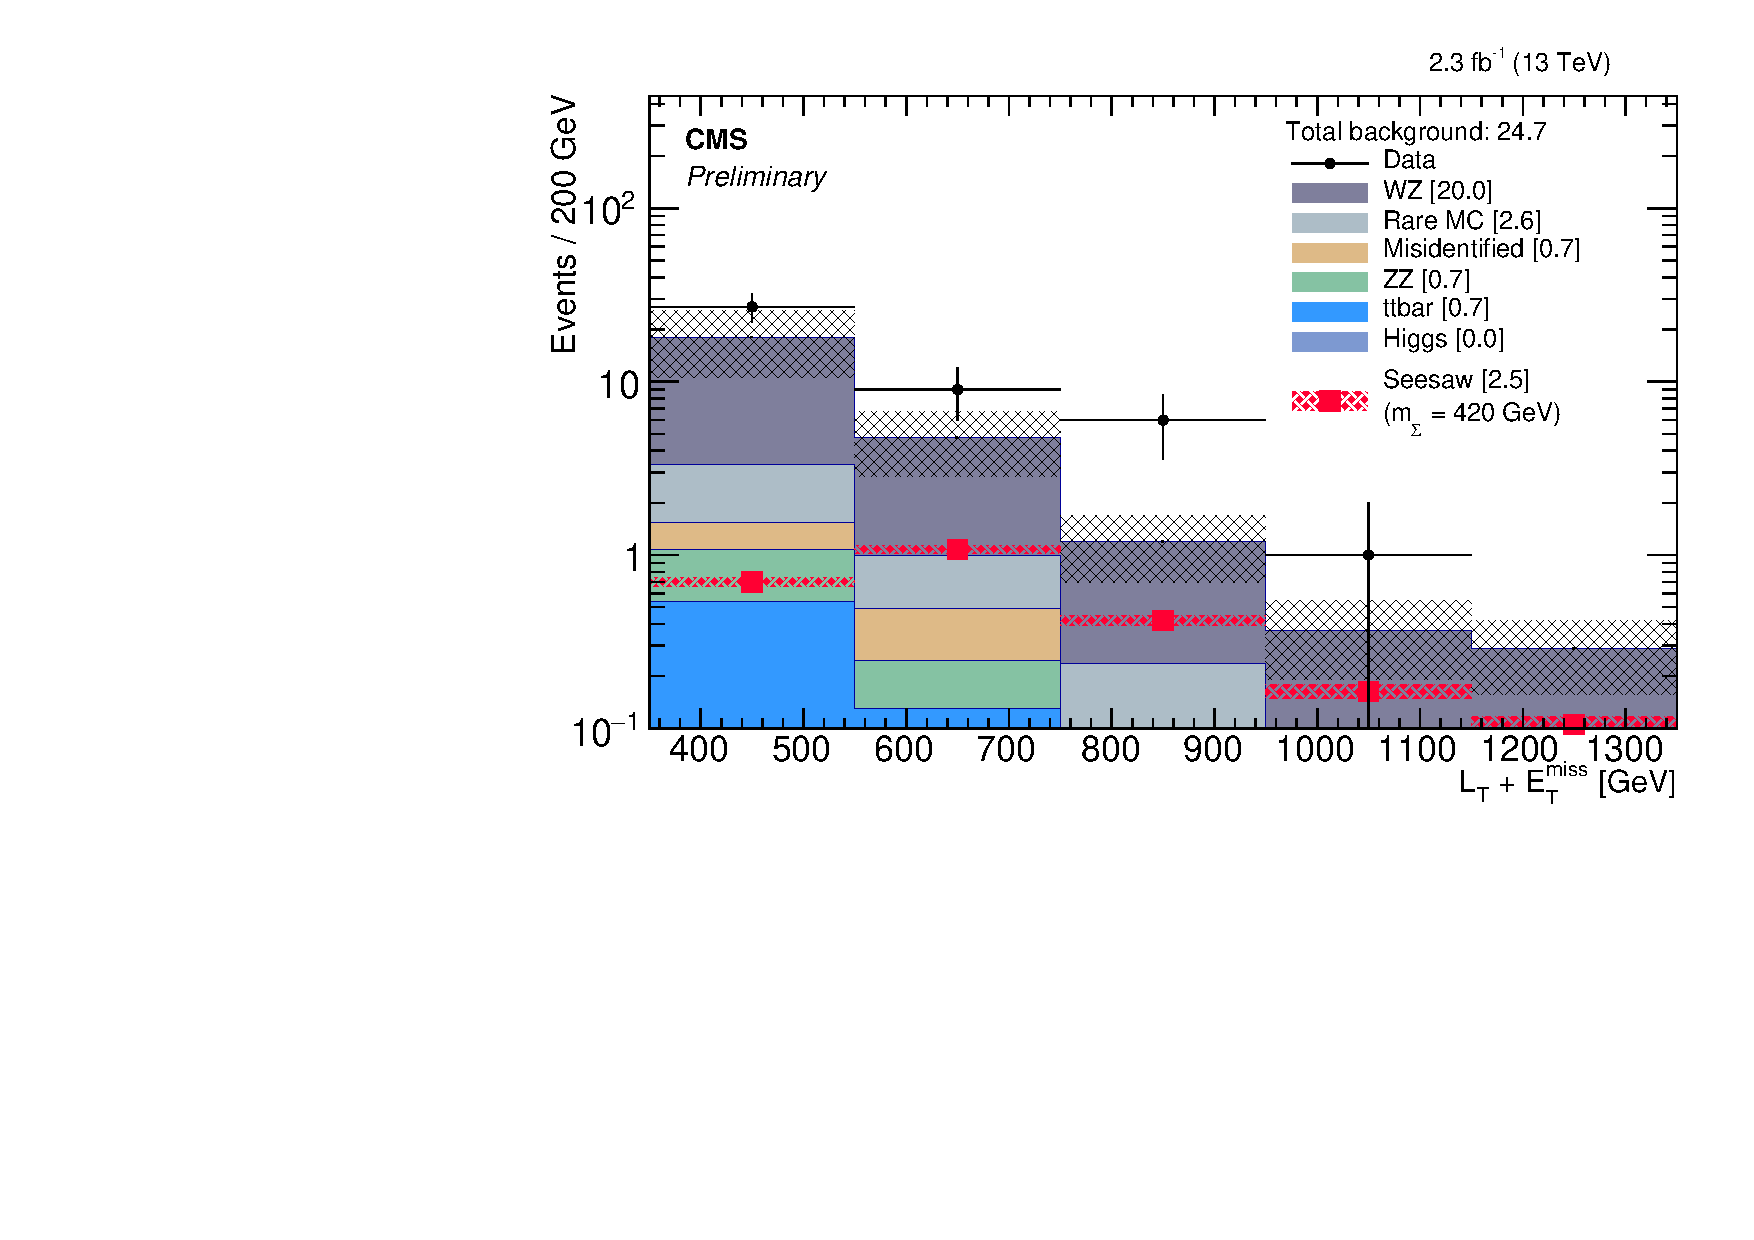
\includegraphics[width=\textwidth]{Results/plots/L3DYz1}
		\caption{3 leptons with OSSF pair on-\Z}
	\end{subfigure}%
	\begin{subfigure}[b]{.5\textwidth}
		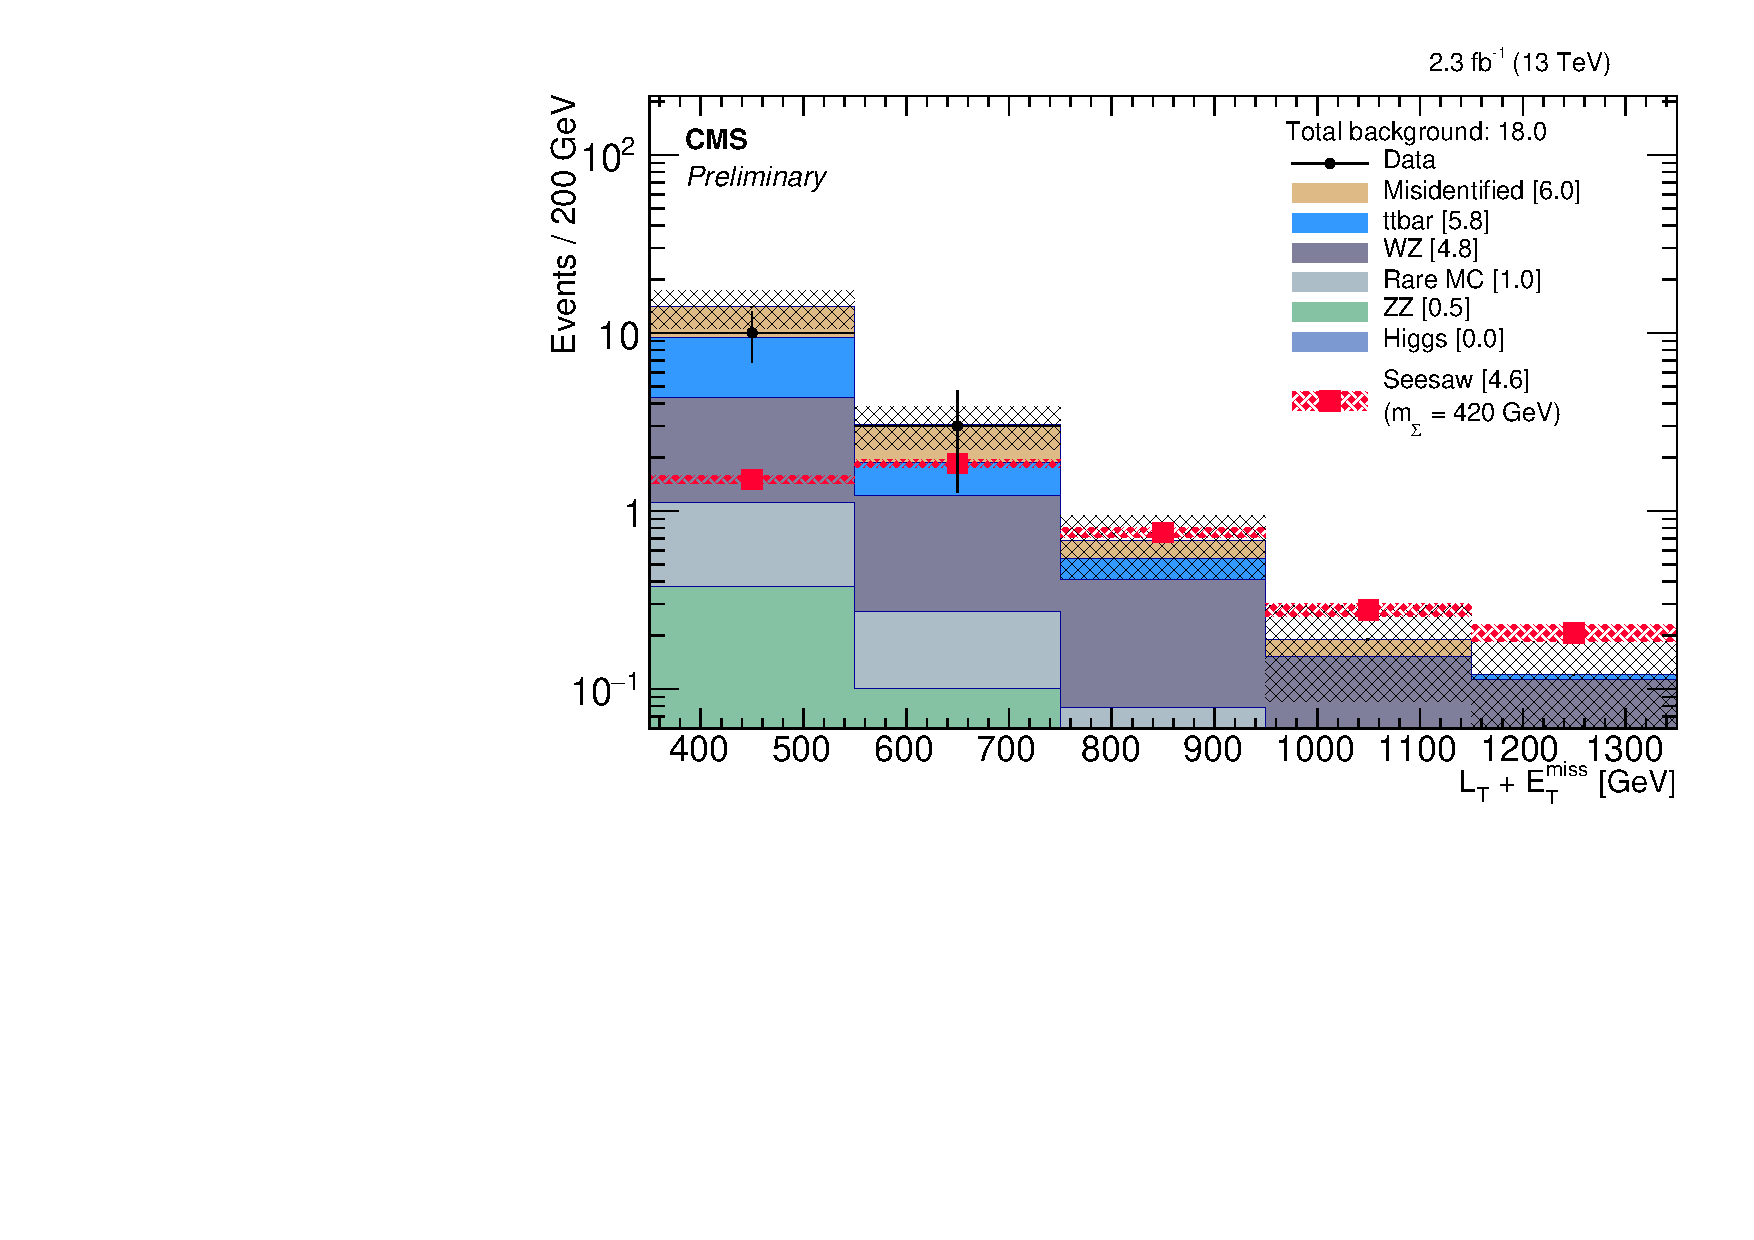
\includegraphics[width=\textwidth]{Results/plots/L3DYh1}
		\caption{3 leptons with OSSF pair above-\Z}
	\end{subfigure}
	\begin{subfigure}[b]{.5\textwidth}
		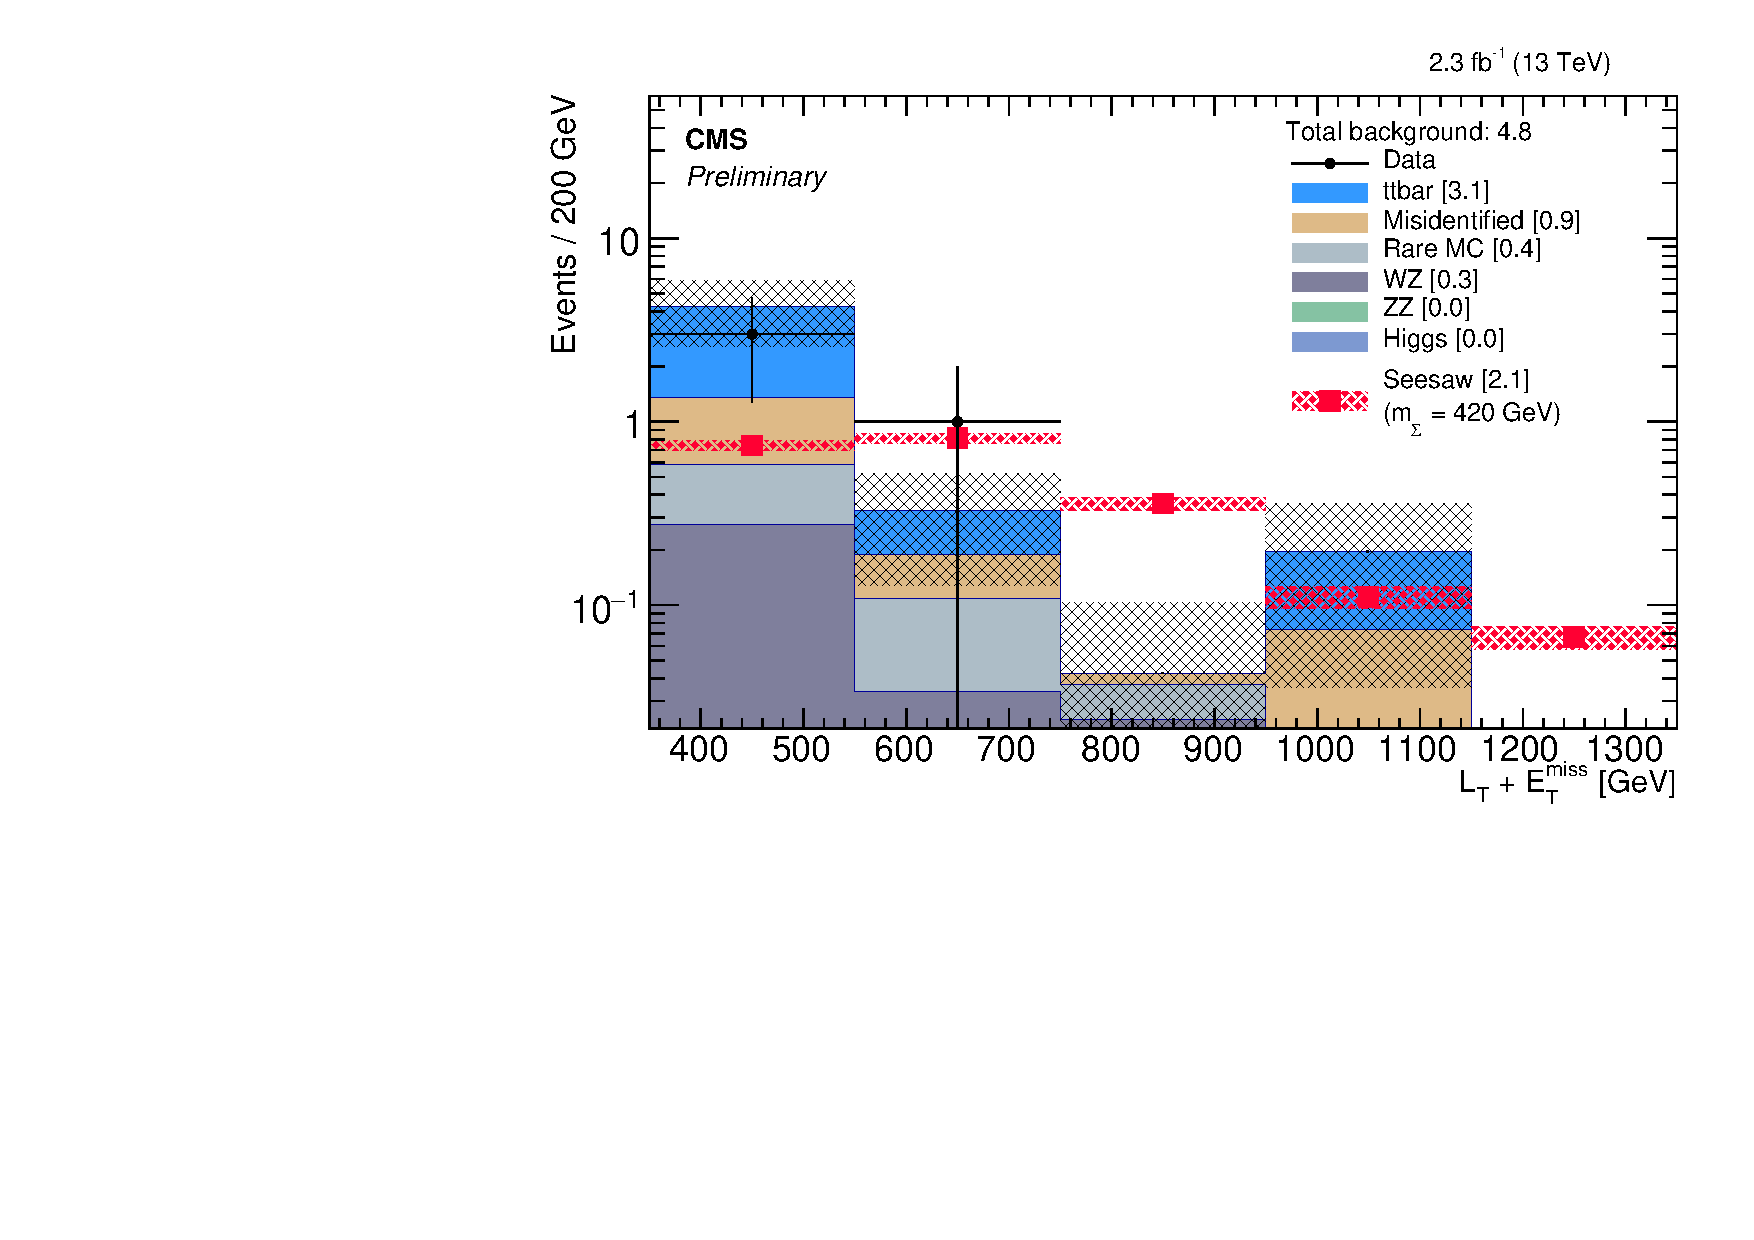
\includegraphics[width=\textwidth]{Results/plots/L3DY0}
		\caption{3 leptons, no OSSF pair}
	\end{subfigure}%
	\begin{subfigure}[b]{.5\textwidth}
		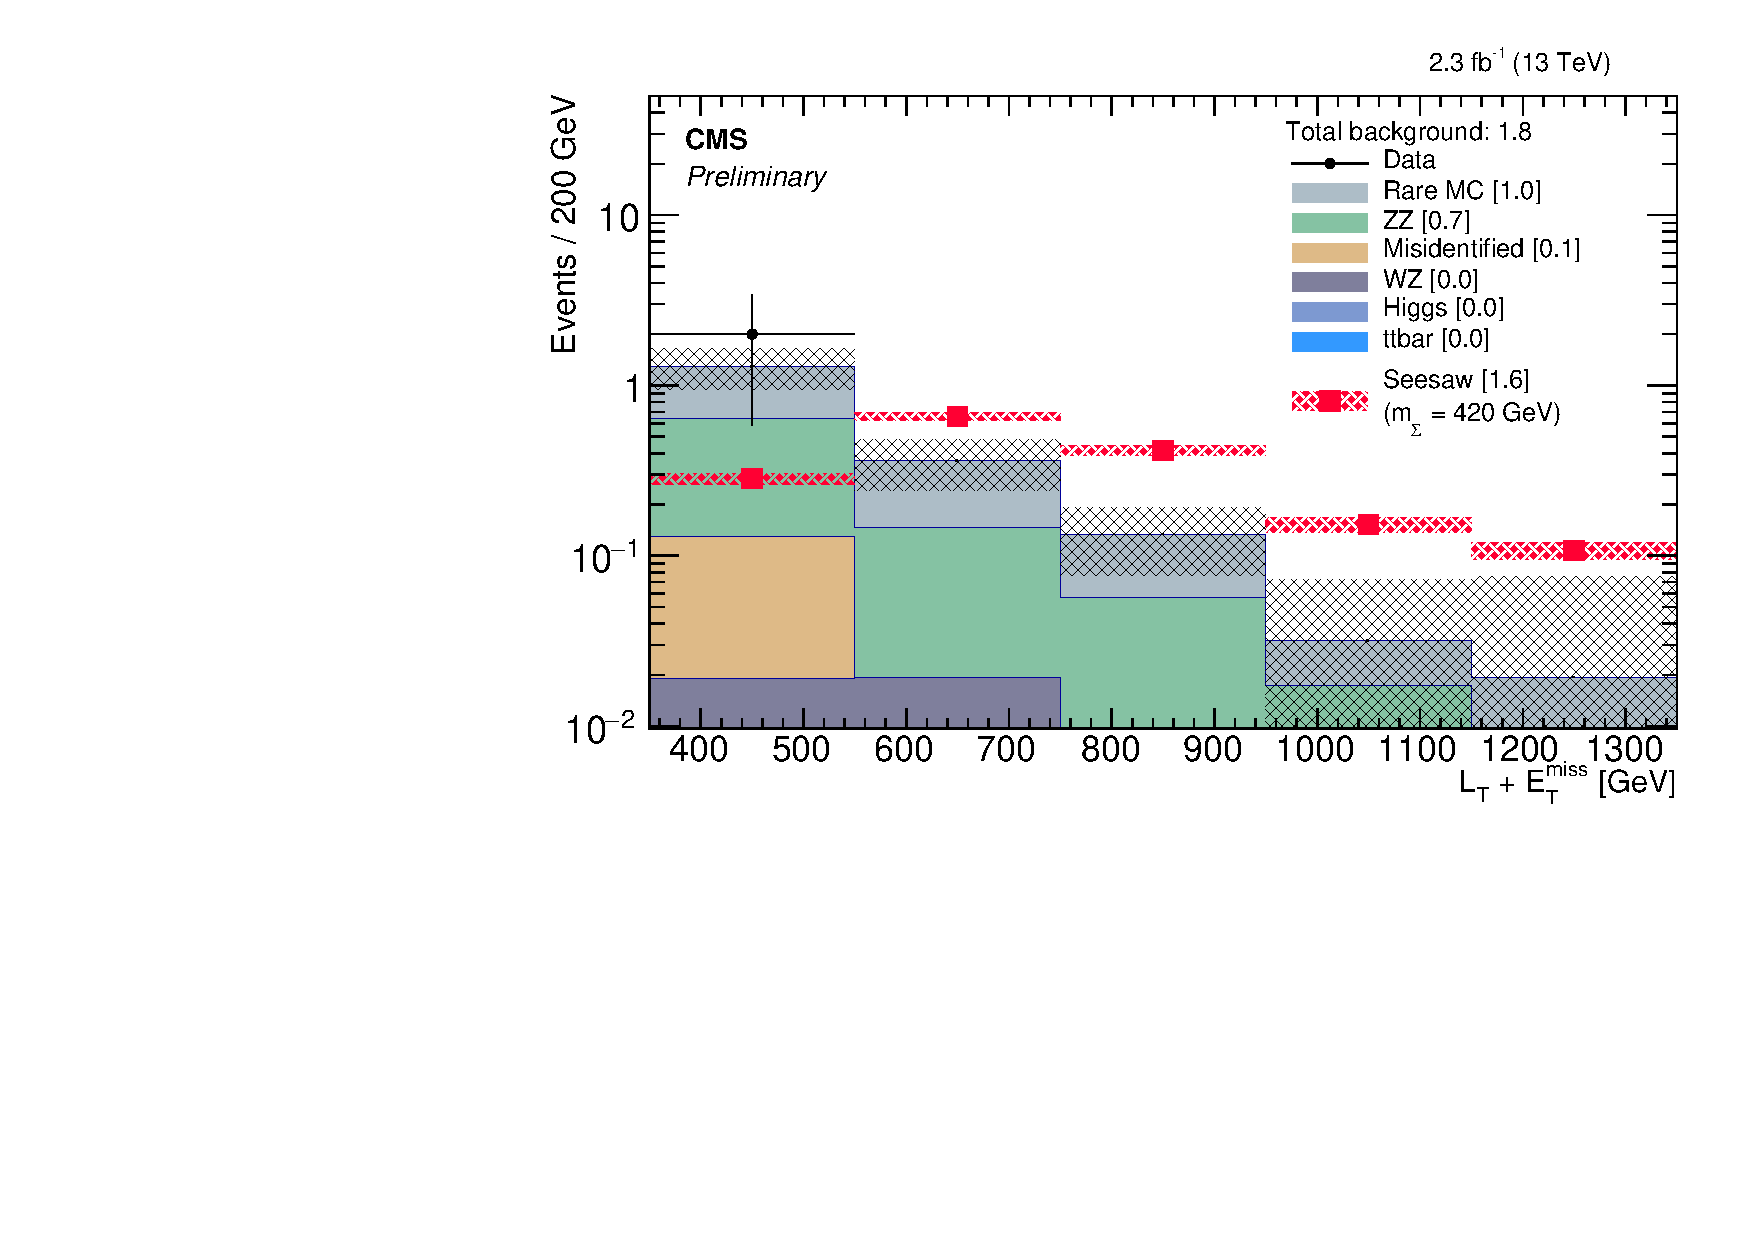
\includegraphics[width=\textwidth]{Results/plots/L4DYgt0}
		\caption{4 leptons, at least 1 OSSF pair}
	\end{subfigure}%
	\caption{Results: $L_\textrm{T} + \MET$ distributions (last bin includes overflow in all plots).
	\label{fig:Results}}
\end{center}
\end{figure}

The observations are consistent with the SM expectations, with the possible exception of the 3-lepton category that includes an OSSF lepton pair with invariant mass consistent with that of the Z boson (Fig.~\ref{fig:Results}a). The dominant background for this category is the \WZ diboson production, as shown. The $p$-value for the hypothesis that the observation in the aggregated twenty $L_\textrm{T} + \MET$ bins for the four categories shown in Fig.~\ref{fig:Results} exceed SM expectation is 0.17. This overall consistency with the SM expectation conveys the message that the apparent excess of observed events in the top-left panel is either a statistical artifact or a discrepancy that can be addressed only with additional data.
